% To build, install TeX-Live, then in this directory,
% pdflatex spark-inequality-impact.tex
% bibtex spark-inequality-impact.aux
% pdflatex spark-inequality-impact.tex
% pdflatex spark-inequality-impact.tex

\documentclass[11pt, oneside]{article}  % use "amsart" instead of "article" for AMSLaTeX format
\usepackage{geometry}
\geometry{letterpaper}                  % ... or a4paper or a5paper or ...
%\geometry{landscape}                   % Activate for for rotated page geometry
\usepackage[parfill]{parskip}           % Activate to begin paragraphs with an empty line rather than an indent
\usepackage{graphicx}                   % Use pdf, png, jpg, or eps with pdflatex; use eps in DVI mode
                                        % TeX will automatically convert eps --> pdf in pdflatex
\usepackage{amsmath}
\usepackage{amssymb}
\usepackage{hyperref}
\usepackage{breakurl}
\usepackage{mathtools}
\usepackage{listings}

\lstset{basicstyle=\small}

\DeclareMathOperator{\Atkinson}{A}
\DeclareMathOperator{\round}{round}

\title{spark-inequality-impact Background}
\author{Stuart Ambler, Guillaume Saint Jacques, Amir Sepehri}
\date{\today}

\begin{document}
\maketitle
\tableofcontents

The spark-inequality-impact software provides a way for economists and others to compute the Atkinson index, a measure of economic inequality, from any Apache Spark DataFrame with a non-negative ``value'' column of double type (not necessarily monetary amounts), using a scala UDAF (user-defined aggregation function) that also gives a ``theoretical'' (asymptotic) variance for the index.  This will scale to large amounts of data.  The software also allows inference on the Atkinson index, including functions to calculate approximate confidence intervals for the index, confidence intervals for the difference of indices from two populations, p-values for the hypothesis that two samples come from populations with the same Atkinson index, and given an Atkinson index value and its $\epsilon$ parameter, an Atkinson-equivalent population of ``haves'' and ``have-nots'', usable as a representative population for that value.

Please see also \cite{SaintJacques} for broader background, more connections and detail.  In particular it gives the asymptotic distribution of the index, which this software uses to calculate an approximate variance.  For background in spark, \cite{Spark} is the documentation for the version of Spark the software has been tested with.  There are many online tutorials.  There are many online references on statistical inference; one that emphasizes the normal approximations we use, which are suitable for large samples, is \cite{Matloff} (see chapter 15 for confidence intervals and section 16.4 for p-values).

\section{The Atkinson inequality index and its $\epsilon$ parameter}

The British economist Anthony B. Atkinson wrote a paper ``On the Measurement of Inequality'' \cite{Atkinson} in 1970 that discusses measures of inequality including the one now named after him, that can be derived from mathematical assumptions about social utility functions and inequality measures.  The Atkinson index summarizes in one number between $0$ and $1$, the inequality of incomes of a group of people.  The value $0$ is attained when everyone has the same income.  Higher values indicate more inequality, and $1$ is an upper bound.

There is an adjustable parameter $\epsilon$, used to indicate how averse to inequality the index will be.  In the spark-inequality-impact software, we assume $0 \le \epsilon < 1$.  It is a choice, with $0$ indicating no aversion to inequality and $1$ indicating considerable aversion; see \cite{SaintJacques} for more on this choice.  \cite{AtkinsonWiki} gives summary information on the Atkinson index and an interpretation of $\epsilon$.

The Atkinson index of inequality with inequality aversion parameter \(\epsilon \) on a sample \(x_1, \ldots, x_n\) is defined by the formula
\[ \Atkinson_\epsilon (x_1, \ldots, x_n) = 1 - \frac{(\frac{1}{n}\sum_{i=1}^n x_i^{1-\epsilon})^\frac{1}{1-\epsilon}}{\frac{1}{n}\sum_{i=1}^n x_i}.\]

An important feature of the Atkinson index method is the fact that it is agnostic to the underlying factors driving inequality, and only measures the inequality in the distribution.

\section{A simple interpretation of the Atkinson index}

Here is a simple way to get a sense of meaning of the actual values of Atkinson indices. The basic idea is to pick, from the infinity of populations with the same Atkinson index (given $\epsilon$), an especially easy to understand representative.

\subsection{Haves and have-nots}

Consider taking the total income for a group of people and dividing it equally among a fraction of them, the ``haves'', leaving the others with no income, the ``have-nots''.  If the fraction is $0$ (no ``haves'') or $1$ (no ``have-nots''), the Atkinson index is $0$ for perfect equality.  Otherwise, if there are relatively few haves, the Atkinson index is large, indicating a lot of inequality, or if relatively many, the index is smaller.  This allows a conversion from the Atkinson index of a group of people (and $\epsilon$), to a representative group with only ``haves'' and ``have-nots'' but with the same Atkinson index.  Below are graphs of the conversion for three values of $\epsilon$.

More technically, let the population size be $N$.  Since the Atkinson index is invariant when all incomes are multiplied by the same positive number, we may as well say that all the ``haves'', whose number is $m$, get $1$ unit of income, and the ``have-nots'', $0$.  Thus we can take the list $x$ of incomes with $m$ equal to $1$ and $N - m$ equal to $0$.  Then the Atkinson index is
\begin{align}
  \Atkinson_{\epsilon)}(x) &= 1 - \frac{(\frac{m}{N})^{\frac{1}{1 - \epsilon}}}{\frac{m}{N}} = 1 - \left(\frac{m}{N}\right)^{\frac{\epsilon}{1 - \epsilon}} \notag
\end{align}
Conversely, if we know the Atkinson index $a$, we can get the fraction $f$ of ``haves'', and obtain their number $m$ to a pretty good approximation since $N$ is fairly large for us, by $m = \round(f N)$.  If $a$ is $1$ we set $f$ to something tiny and $m$ to $1$.  Otherwise,
\begin{align}
  f &= (1 - a) ^ \frac{1 - \epsilon}{\epsilon} \notag
\end{align}

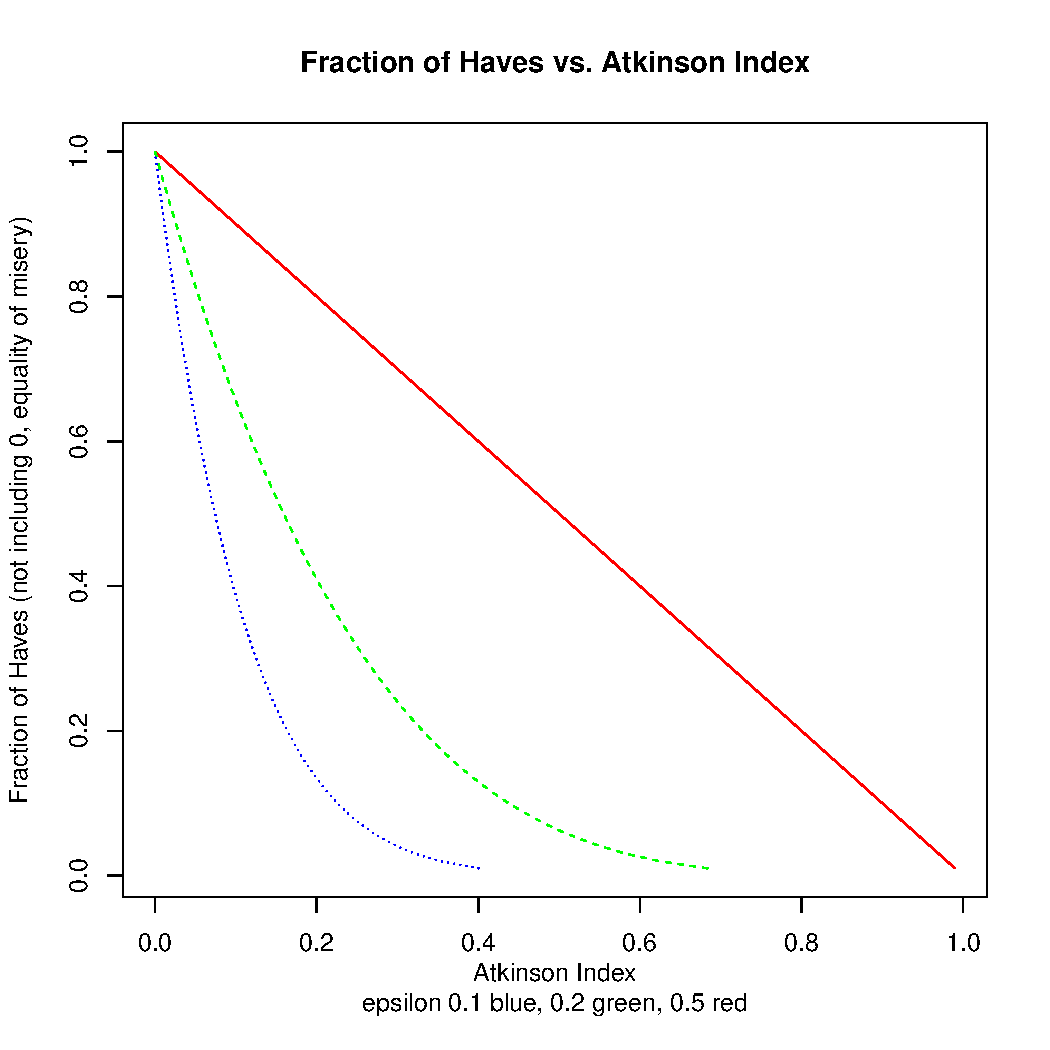
\includegraphics[scale=0.5]{../R/atkinson-to-haves.pdf}

\subsection{Comparison of pairs of Atkinson indices using haves}
It may be important to compare Atkinson indices for pairs of groups, such as from A/B tests.  Each of the Atkinson indices can be converted to a fraction, and then the fractions subtracted.  The interpretation, for example of ``the Atkinson-equivalent fraction of haves increased by 0.1'' would be that splitting up the income equally among a group of haves of the size that corresponds to the Atkinson index, both before and after an intervention, the fraction of haves increased by $0.1$.

\subsection{Variance of number and fraction of haves in a random sample}
Suppose that we sample $r$ elements at random from a population of size $N$ that actually has $h$ haves. Then following \cite{Feller} pages 232-233, the number of haves in the sample has a hypergeometric distribution with expected value $r h / N$ and variance $r h (N - h) (N - r) / (N^2 (N - 1))$.  Letting $f = h / N$ denote the fraction of haves in the population,
\begin{align}
  \text{Expected fraction of haves in sample} &= f \notag \\
  \text{Variance of fraction of haves in sample} &= f (1 - f) \frac{N - r}{N - 1} \notag
\end{align}
(The factor $(N - r) / (N - 1)$ would be omitted if the sampling were with replacement.)  To compute confidence intervals for the haves fraction, one can use R package hypersamplan, or e.g. the online calculator at \url{https://epitools.ausvet.com.au/ciproportion}.

In a simulation drawing samples of size $2$K from a population of size $20$K with $20$\% $1$s and the rest $0$s, the actual and calculated variances agreed within $1.4$\%.  For a gamma distribution with shape parameter 0.114 (sharply peaked) the agreement was within $13$\%.  For lognormal data, the ratio of actual to calculated was $15$ in one run; the numbers varied from run to run.

\section{A way to think  of  Atkinson index differences in terms of CDFs}

Here is theoretical background giving a way to think of the difference of two Atkinson indices, in terms of the distributions of the populations.  The population value of the Atkinson index is

\[ \Atkinson_\epsilon(F) = 1 - \frac{\left(\int x^{1-\epsilon} dF(x) \right)^{\frac{1}{1-\epsilon}}}{\int x dF(x)} \]

Since the Atkinson index is scale invariant, we can assume \(\int x dF(x) = 1\). Then, we can compare the Atkinson index for two populations with CDFs \(F\) and \(G\) using the following heuristic:

\[\Atkinson_\epsilon(F)  - \Atkinson_\epsilon(G)  \approx \left(\int x^{1-\epsilon} dG(x) \right)^{\frac{\epsilon}{1-\epsilon}}  \left(\int x^{-\epsilon} (G(x)- F(x)) d x \right)\].

What this means is that the difference between the distribution at \(x\) is weighted by \(x^{-\epsilon}\). This weights the difference at the lower part of the population more heavily than the upper part. The difference in the weighting depends on \(\epsilon\). The following derivation justifies the approximation.

For two populations with CDFs \(F\) and \(G\) we have

\[  \Atkinson_\epsilon(F)  - \Atkinson_\epsilon(G) = \left(\int x^{1-\epsilon} dG(x) \right)^{\frac{1}{1-\epsilon}} - \left(\int x^{1-\epsilon} dF(x) \right)^{\frac{1}{1-\epsilon}} \]

A Taylor expansion of the function \(f(x) = x^{\frac{1}{1-\epsilon}} \) yields

\[\Atkinson_\epsilon(F)  - \Atkinson_\epsilon(G)  \approx \frac{1}{1-\epsilon} \left(\int x^{1-\epsilon} dG(x) \right)^{\frac{\epsilon}{1-\epsilon}}  \left(\int x^{1-\epsilon} dG(x) - \int x^{1-\epsilon} dF(x) \right) \]

Using integration by parts we get the result.

\medskip

\addcontentsline{toc}{section}{References}
\bibliography{spark-inequality-impact}{}
\bibliographystyle{alpha}

\end{document}
